\documentclass{beamer}

\usepackage{listings}
\usepackage{color}

\definecolor{dkgreen}{rgb}{0,0.6,0}
\definecolor{gray}{rgb}{0.5,0.5,0.5}
\definecolor{mauve}{rgb}{0.58,0,0.82}

\lstset{frame=tb,
  language=Haskell,
  aboveskip=3mm,
  belowskip=3mm,
  showstringspaces=false,
  columns=flexible,
  basicstyle={\small\ttfamily},
  numbers=none,
  numberstyle=\tiny\color{gray},
  keywordstyle=\color{blue},
  commentstyle=\color{dkgreen},
  stringstyle=\color{mauve},
  breaklines=true,
  breakatwhitespace=true,
  tabsize=3
}

\usepackage{amsmath}
\usepackage{amssymb}
\usepackage{tikz}

\usetheme{CambridgeUS}
\setbeamertemplate{caption}[numbered]


\AtBeginSection[]{
\begin{frame}
	\vfill
	\centering
	\begin{beamercolorbox}[sep=8pt,center,rounded=true,shadow=true]{title}
	  {\usebeamerfont{title}\insertsectionhead}\par%
	\end{beamercolorbox}
	\vfill
\end{frame}
}
  

\title{Inference \& Evaluation Engine for Feed-Forward Neural Networks}
\subtitle{CS-IS-2010-1 Final Project}
\author{Santripta Sharma}
\date{\today}

\begin{document}

\begin{frame}
	\titlepage
\end{frame}	

\begin{frame}{Introduction}
  \begin{itemize}
    \item Through the course of the semester, I have developed a command-line tool to run inference on (or evaluate) an arbitrary feed-forward network classifier.
    \item The entire process took me from the basics, performing command-line I/O, and using the haskell tool stack, all the way to writing binary data parsers, using monads, and implementing test suites with HSpec.
    \item<2-> Besides these learning outcomes, the tool has been designed \& implemented to maximise optimality, generalizability, and usability.
  \end{itemize}
\end{frame}

\begin{frame}{Motivation}
  \begin{itemize}
    \item Machine Learning has left no domain/sector untouched.
    \item<2-> Problem: A large chunk of the users of ML models are not familiar with how
    they work or how to use them.
    \item<2-> Widespread black-boxing: development/training of the model is outsourced to someone with this technical knowledge
    \item<2-> Besides security risks, also leaves the non-savvy client at the vendor's mercy
    \item<3-> Requirement of a trusted solution to self-validate vendor's claims about model accuracy
  \end{itemize}
\end{frame}

\section{Background \& Literature Survey}
\begin{frame}{Feed-Forward Neural Networks}
  \begin{center}
    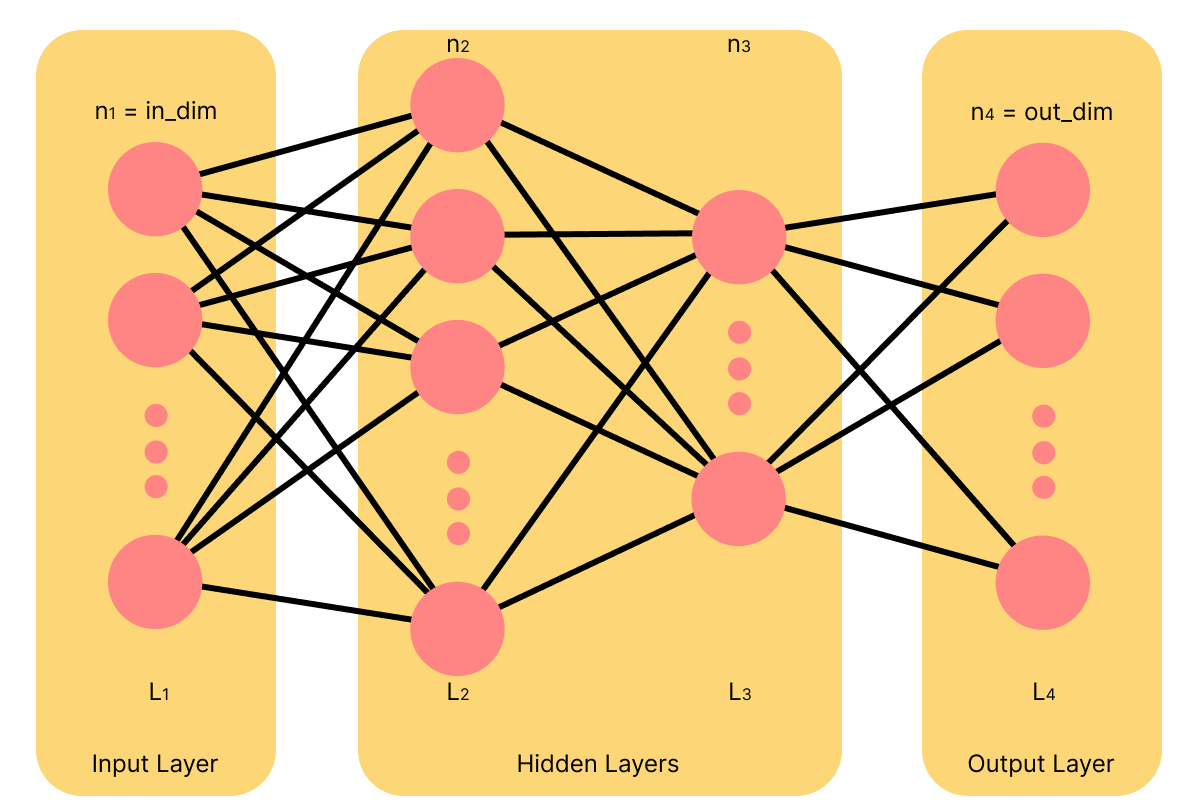
\includegraphics[width=0.9\textwidth]{../images/FFN-Structure.png}
  \end{center}
\end{frame}

\begin{frame}{Feed-Forward Neural Networks}
  Propagation formula (for $2 \leq i \leq n_{layers}$):
  \begin{align*}
    X_i = &\text{Activation}(W_iX_{i - 1} + B_i)
  \end{align*} 

  \begin{lemma} \label{lem:1}
    Given the weights matrix $W_i: a \times b$ at layer $L_i$, we have that $n_{i - 1} = b$.
  \end{lemma} \label{lem:2}
  \begin{lemma}
    Given the weights matrix $W_i: a \times b$ at layer $L_i$, we have that $n_i = a$.
  \end{lemma}
  \begin{lemma} \label{lem:3}
    Given the weights matrix $W_i: a \times b$ at layer $L_i$, the biases vector $B_i$ has the shape $B_i: a \times 1$.
  \end{lemma}
\end{frame}

\begin{frame}{Existing Neural Network Libraries}
  \begin{itemize}
    \item We want to avoid reinventing the wheel.
    \item Several neural network libraries exist for haskell: neural, grenade, hnn, neural-network-hmatrix
    \item All share the same issue: too general
    \item Focused on training + inference, trade simplicity for generality
    \item<2-> Time to reinvent the wheel. Where do we begin?
  \end{itemize}
\end{frame}

\begin{frame}{Fast Linear Algebra in Haskell}
  \begin{table}\label{tab:1}
    \centering \begin{tabular}{|c|c|c|c|}
      \hline \textbf{Library} & $n = 10$ & $n = 50$ & $n = 100$\\
      \hline DLA & 2.65us & 289.0us & 2.24ms\\
      \hline Hmatrix & 1.32us & 55.8us & 292.0us\\
      \hline NumHask & 714.0us & 63.5ms & 593.0ms\\
      \hline Massiv & 12.0us & 205.0us & 1.52ms\\
      \hline Massiv (Parallel) & 76.1us & 220.0us & 866.0us\\
      \hline Matrix & 12.6us & 1.1ms & 8.44ms\\
      \hline Naive C Implementation & 51us & 323us & 4.78ms\\
      \hline
    \end{tabular}
  \end{table}  
  \begin{itemize}
    \item To do fast neural network inference, do fast matrix multiplication and addition
    \item Many linear algebra libraries: matrix, DLA, massiv, hmatrix, numhask
    \item The table above shows a benchmark from 2015, for matrix multiplication of size $n\times n\times n$
    \item<2-> Conclusion: use hmatrix
  \end{itemize}
\end{frame}

\section{Problem Definition \& Objectives}

\begin{frame}{Problem Statement}
  \begin{block}<1->{Problem Statement}
    Develop a classification model over the Iris Dataset and store the model. Then write a Haskell code to restore the model, input new data (based on the four features of the iris) and generate a prediction in real time.
    \begin{enumerate}
      \item<2-> Input: The Iris Dataset.
      \item<2-> Output: Real-time prediction for the class of the flower of a new data row containing the sepal width, petal width, sepal length and petal length.
      \item<3-> Method: You can use Python to train and save a classification model (SVM or NN). However, restoring the model and the real-time prediction of a new data row has to be written only in Haskell.
    \end{enumerate}
  \end{block}
\end{frame}

\begin{frame}{Objectives}
  Based on this statement \& the motivation, we set our objectives:
  \begin{block}<1->{Objectives}
    Develop a system which:
    \begin{itemize}
      \item Can load a trained FFN-based classification model.
      \item Can make predictions on an unseen/new datapoint belonging to the same dataset.
      \item Is as performant as possible, since the problem description suggests that the application domain is a real-time system.
      \item Is simple to use for a layperson.
      \item Generalises beyond the iris dataset.
      \item Can evaluate the given model in some capacity
    \end{itemize}
  \end{block}
\end{frame}

\begin{frame}{Scope}
  We have developed a system with the following featureset:
  \begin{enumerate}
    \item Parsing capabilities to restore the shape, weights, and biases of \textbf{an arbitrary} FFN classifier from a file on disk.
    \item Interactive \& batched modes of performing inference. \begin{itemize}
      \item \textbf{Interactive}: The user enters a single new datapoint and gets predictions for it in real-time. Structured as a Read-Eval-Print-Loop (REPL).
      \item \textbf{Batched}: The user provides many datapoints in a csv file, and receives predictions for each point.
    \end{itemize}
    \item An evaluation mode: an extension of batched inference mode which also takes in expected outputs, and determines model accuracy.
  \end{enumerate}
  We limit the class of models we allow to using ReLU (at the hidden layers) \& Softmax (at the output layer) activations.
\end{frame}

\section{System Design \& Methodology}
\begin{frame}{High-level view}
  \begin{figure}
    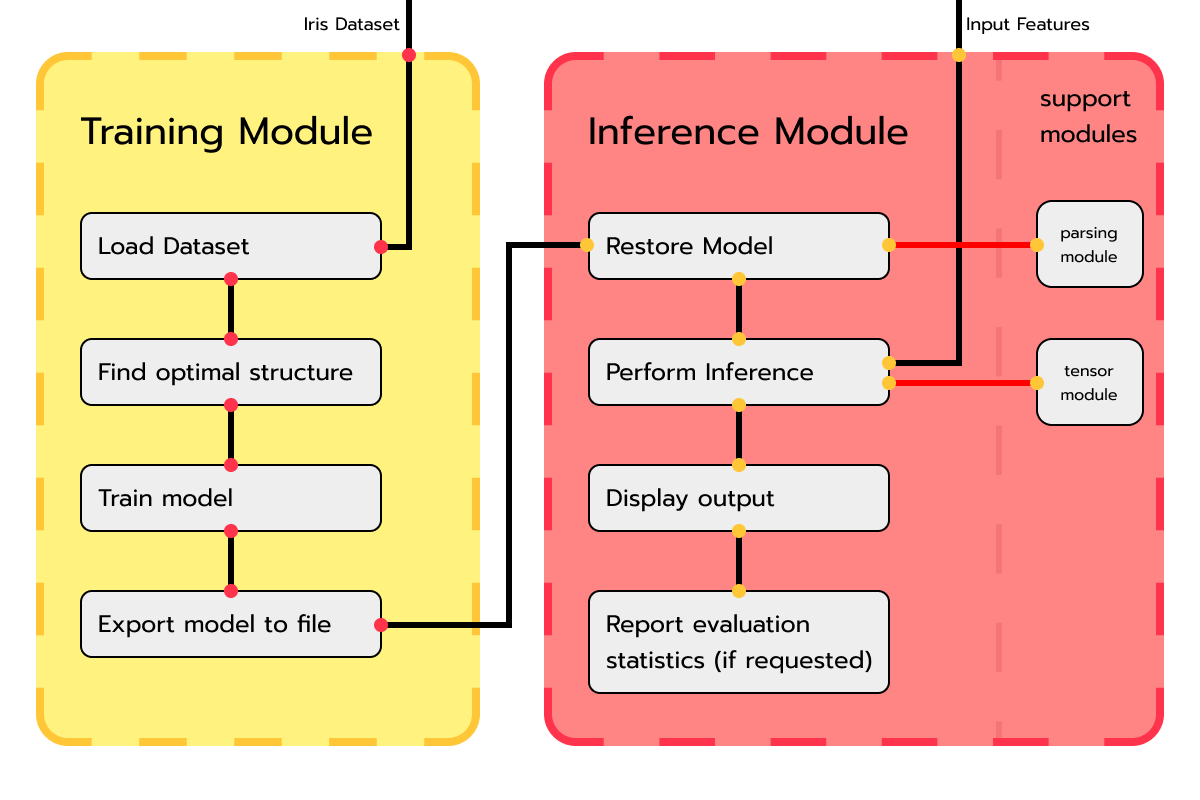
\includegraphics[width=0.95\textwidth]{../images/modules.png}
  \end{figure}
  \only<2>{%
  \tikz[overlay,remember picture]
  \node[fill=blue,text=white,rotate=90] at ([xshift=-0.8cm,yshift=-0.9cm]current page.center){what's happening here?};
  }
\end{frame}

\begin{frame}[fragile]{Trained Model Format}
  We use a custom binary format to store our trained models.
  
  A naive implementation of such a format goes as follows:
  \begin{verbatim}
number of layers
for each non-input layer in the network:
  weights matrix rows
  weights matrix columns
  weights matrix
  biases vector length
  biases vector
  \end{verbatim}
  Since each integer stored is 4-bytes, this requires $4(3l + 1) + D$ bytes to store, where $D$ is the constant size of the data (weights \& biases), and $l$ is the number of layers.
\end{frame}

\begin{frame}[fragile]{Trained Model Format}
  Using our lemma, we can infer the biases vector length from the weights matrix rows:
  \begin{verbatim}
number of layers
for each non-input layer in the network:
  weights matrix rows
  weights matrix columns
  weights matrix
  biases vector
  \end{verbatim}
  This requires $4(2l + 1) + D$ bytes to store
\end{frame}

\begin{frame}[fragile]{Trained Model Format}
  Using our other lemma, we can infer the weights matrix columns from the previous weights matrix rows (i.e. number of neurons in previous layer):
  \begin{verbatim}
number of layers
number of neurons in input layer
for each non-input layer in the network:
  weights matrix rows
  weights matrix
  biases vector
\end{verbatim}
  This requires $4(l + 2) + D$ bytes to store, which scales much better with number of layers, and since we iteratively parse layer after layer, we can memoise the previous layer's neuron count to determine the number of columns in any layer's weights matrix.

  We store the number of neurons in the input layer for initialisation.
\end{frame}

\begin{frame}
  \frametitle{Training Module}

  \begin{itemize}
    \item The training module provides us with a set of models we can use to test our inference module.
    \item<2-> Using a 5-fold cross-validation, we perform a grid search to find the best 5 network shapes for the architecture mentioned above, as well as the worst shape.
    \item<3-> We then train these 6 models on a split of the dataset, and save them to disk in the format discussed above. Additionally, we train a large 12-layer model to be used for benchmarking.
  \end{itemize}

\end{frame}

\begin{frame}[fragile]
  \frametitle{Inference Module}

  \begin{itemize}
    \item The inference module produces an executable with the following signature: \verb|inference-exe <path_to_model_file> [<path_to_batch_csv>]| 
    
    \verb|[path_to_ground_truth]|

    If no optional arguments are given, it starts in interactive mode, if the batch csv is provided it starts in batch mode, and if the ground truth csv is provided, it starts in evaluation mode.
    \item<2-> It first restores the model from the given model file, utilising the parsing support module.
  \end{itemize}
\end{frame}

\begin{frame}{Inference Module}
  \begin{itemize}
    \item Then, based on which mode it was started in, it collects user input accordingly, and uses the tensor support module to perform the inference. If it was started in interactive or batched mode, it reports the output activations and class labels, otherwise it reports \% accuracy and the number of correct predictions.
  \end{itemize}
\end{frame}

\section{Work Done}

\begin{frame}
  \frametitle{Tooling}

  \textbf{Training Module}\\
  The training module is written in \textbf{python}, using \textbf{numpy}, \textbf{pandas}, and \textbf{sklearn} to perform the data processing \& model training/selection.\bigskip

  \textbf{Inference Module}\\
  The inference module is written in \textbf{Haskell}. We use the \textbf{Haskell Tool Stack} (or just Stack) as our build tool. The following libraries are used:
  \begin{itemize}
    \item \textbf{hmatrix}
    \item \textbf{cereal}
    \item \textbf{cassava}
  \end{itemize}
\end{frame}

\begin{frame}{Tooling}
  \textbf{Misc/Testing}\\
  A mix of bash \& python scripts is used to implement the end-to-end tests and certain convenience utilities. Additionally, we use HSpec for unit testing \& timeit for benchmarking performance.
\end{frame}

\subsection{Test Suite}

\begin{frame}
  \frametitle{Testing Strategy}
  
  Due to the large number of disjoint moving parts in the project, the plan is to implement a comprehensive test suite consisting of unit \& end-to-end tests. Additionally, we will be profiling our system to ensure it meets the real-time requirements.\bigskip

  Unit tests are implemented using \textbf{HSpec}, the testing framework provided by \textbf{Stack}.
\end{frame}

\begin{frame}
  \frametitle{Unit Testing}

  First, we note that the training module does not require testing, due to its simplicity and it almost exclusively using sklearn library functions.\medskip
  
  For the inference module, the inference functions are complex enough to warrant unit testing.
  
  As it stands, the batch inference function is tested by the end-to-end test. Therefore, we focus our attention on the single-row inference function.
\end{frame}

\begin{frame}
  \frametitle{Unit Testing}

  Using HSpec, the default testing framework included with the Haskell stack, we test this function for four cases:
  \begin{itemize}
    \item Empty Network: Should throw an error
    \item Invalid Input Dimensions: Should throw an error
    \item Invalid Network Configuration: Should throw an error 
    \item Correct Functioning: Use randomly generated valid inputs to check our function output against the explicit formula.
  \end{itemize}
\end{frame}

\begin{frame}
  \frametitle{E2E Testing}
  \begin{center}
    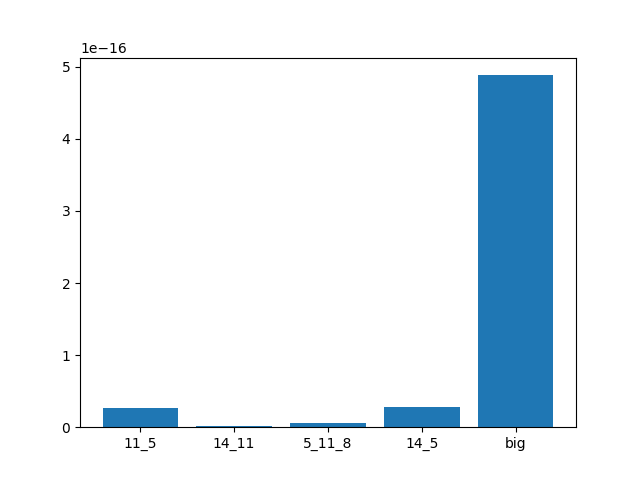
\includegraphics[width=0.8\textwidth]{../images/mse.png}
  \end{center}
\end{frame}

\begin{frame}
  \frametitle{Profiling}
  \begin{center}
    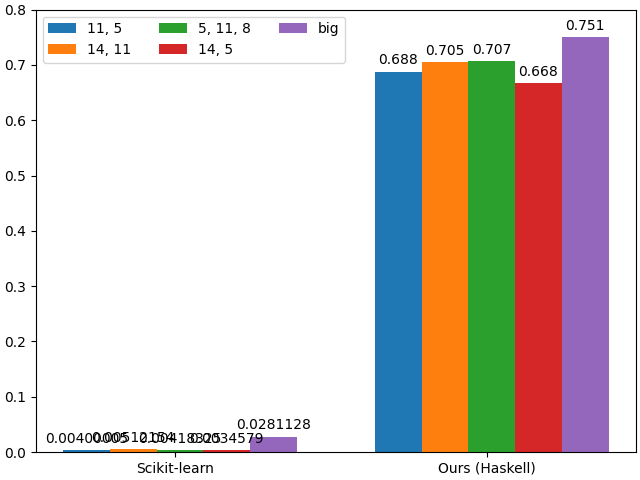
\includegraphics[width=\textwidth]{../images/benchmark.png}
  \end{center}
\end{frame}

\subsection{Implementation}

\begin{frame}
  \frametitle{Functionality/User Flow}

  \begin{center}
    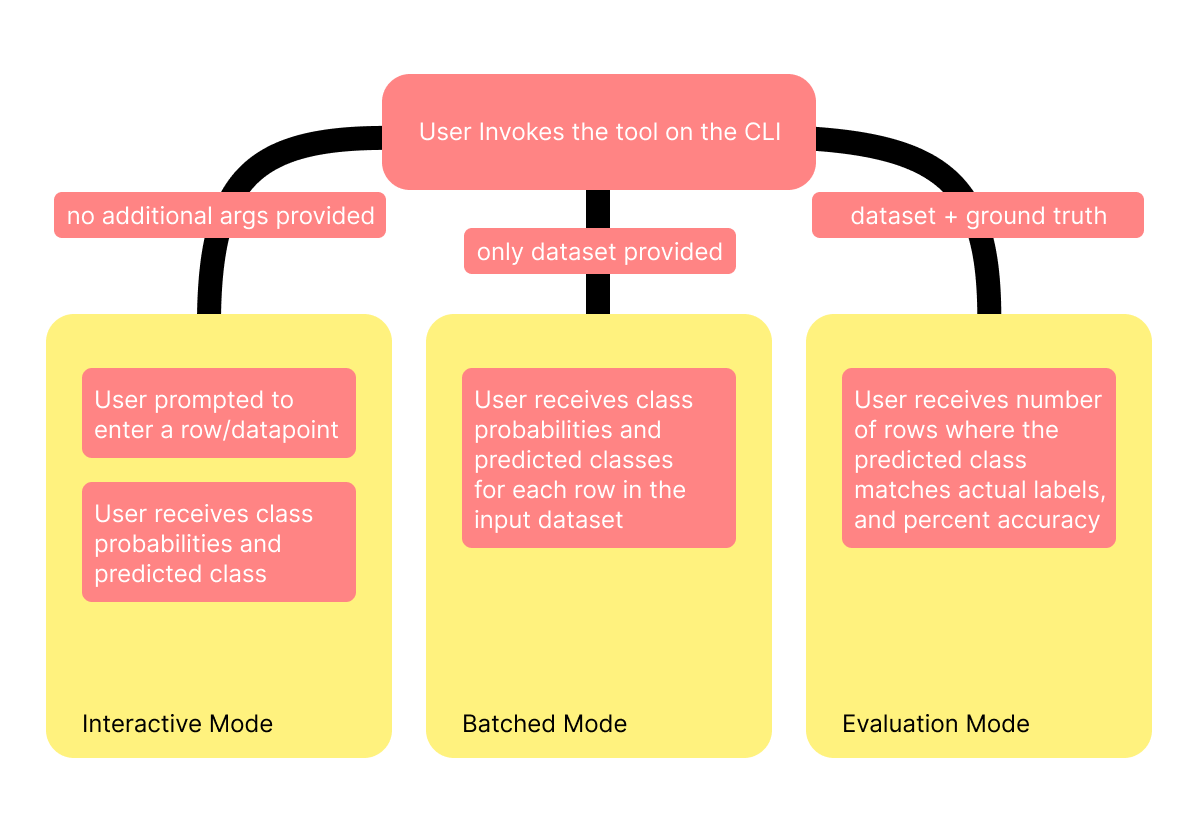
\includegraphics[width=0.9\textwidth]{../images/UserFlow.png}
  \end{center}
\end{frame}

\begin{frame}
  \frametitle{Examples}
  \begin{figure}
    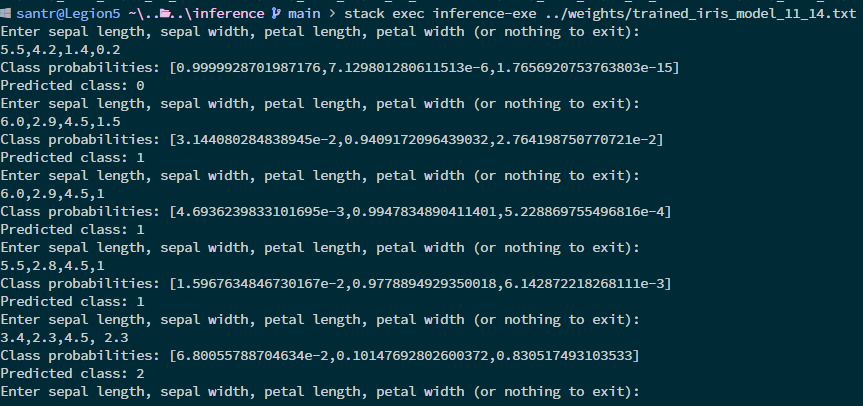
\includegraphics[width=0.9\textwidth]{../images/examples.png}
    \caption{examples of inference in interactive mode}
  \end{figure}
\end{frame}

\begin{frame}
  \frametitle{Examples}
  \begin{figure}
    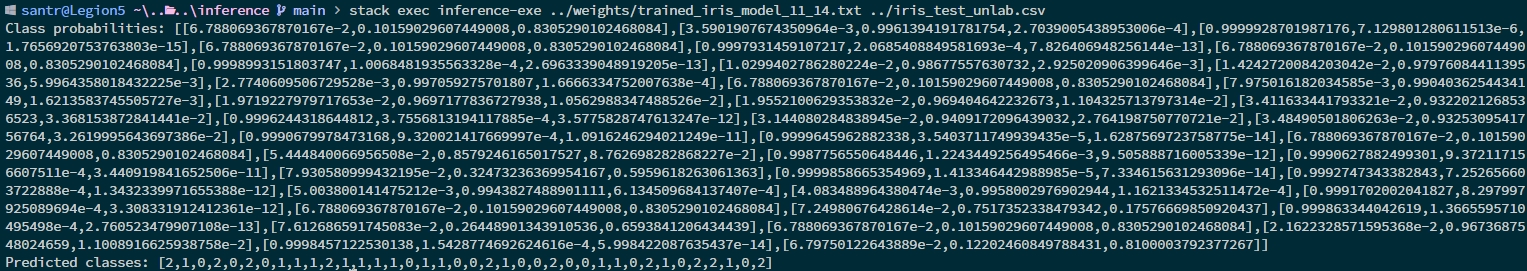
\includegraphics[width=\textwidth]{../images/examplebatch.png}
    \caption{example of inference in batched mode}
  \end{figure}
\end{frame}

\begin{frame}
  \frametitle{Examples}
  \begin{figure}
    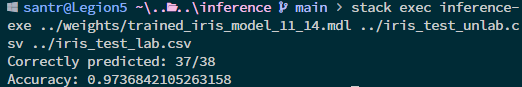
\includegraphics[width=0.9\textwidth]{../images/exampleeval.png}
    \caption{example of evaluation mode}
  \end{figure}
\end{frame}

\subsection{Challenges \& Pitfalls}

\begin{frame}
  \frametitle{Challenges \& Pitfalls}

  While designing and implementing the project, I ran into several pitfalls, including but not limited to:
  \begin{itemize}
    \item \textbf{Migrating Libraries from Midterm}
    \item \textbf{Configuring LAPack \& Blas}
    \item \textbf{Initial Benchmarks}
  \end{itemize}
\end{frame}

\begin{frame}
  \frametitle{Migrating Libraries from Midterm}

  \begin{itemize}
    \item During the final stage of the project, we made several migrations to different libraries. Some planned, some unplanned.
    \item Even the planned migration from parsec to attoparsec did not go to plan, attoparsec doesn't support parsing IEEE754 numbers correctly
    \item Later, we found cereal, and despite migration to it being smooth, a lot of time was lost in the process.
    \item<2-> A less smooth transition was seen after completing our literature survey and finding hmatrix.
    \item<2-> Required a rewrite of our entire inference codebase, to fit hmatrix's interface.
  \end{itemize}
\end{frame}

\begin{frame}
  \frametitle{Configuring LAPack \& Blas}

  \begin{itemize}
    \item hmatrix owes most of its speed gains to it essentially being a wrapper for the industry standard numerical linear algebra packages, LAPack \& Blas.
    \item Once the inference module had been rewritten for hmatrix, it no longer compiled, leading us down a deep rabbithole of dependency management.
    \item Only old and unreliable answers available online.
    \item Eventually, the Haskell Tool Stack documentation revealed that on windows, it maintains its own MSYS2 environment for this purpose.
    \item Big time sink.
  \end{itemize}

\end{frame}

\begin{frame}[fragile]
  \frametitle{Initial Benchmarks}

  \begin{itemize}
    \item In our initial benchmarks, even after the migration to hmatrix, we observed less than ideal results.
    \item Problem narrowed down to one line of code: \verb|col = (toColumns mat) !! colIdx|
    \item<2-> Replacing this with \verb|col = flatten $ mat ? [colIdx - 1]| immediately led to a 4x speedup.
    \item<2-> The pitfalls of interoperation.
  \end{itemize}

\end{frame}

\section{Discussion \& Conclusion}

\begin{frame}
  \frametitle{Limitations}
  \begin{itemize}
    \item The command-line interface, while designed for usability, still may serve as a barrier for the most technically-challenged individuals
    \item Requires the weights to be in a particular format
    \item During interactive inference, invalid inputs are not handled gracefully
    \item Class labels aren't currently considered, which hinders readability
    \item The system's performance, while optimised, fails to compete with sklearn's.
  \end{itemize}
\end{frame}

\begin{frame}
  \frametitle{Conclusions}
  We have built a successful baseline inference package using haskell, though it is clear that it is far from complete. Besides lacking many configuration options and flexibility, it also fails to achieve the performance one would expect from a more standard package implemented in python with something like sklearn. Nonetheless, we have developed an accurate and acceptably performant system for inferencing feed-forward network classifiers.
\end{frame}

\begin{frame}
  \frametitle{Conclusions}
  Further, we have expanded the scope of the project from the intial problem statement to provide a more general solution than was expected. In doing so, we have also provided a partial solution to the black-boxing problem discussed in our motivation.\bigskip

  Finally, we were able to propose a specialised format for serializing trained feed-forward classifiers, which is space effective and utilises our understanding of the network architecture to achieve this optimisation.
\end{frame}

\begin{frame}
  \frametitle{Extensions \& Future Work}

  \begin{itemize}
    \item Infer the format of the weights file based on a few well-known formats (.pkl, .pth, .safetensors), instead of only working for our custom format. This requires more than just looking at the extension, as we have to further infer where the weights and biases of each layer lie based on the keys in the file. 
    \item<2-> The inference performance should be inspected more deeply and optimised accordingly.
    \item<3-> Currently, we have not performed any profiling on the parser, which is a core component of the entire system.
    \item<4-> A graphical user interface could greatly enhance the program's usability.
    \item<5-> Model input space could be extended to accept more architectures, such as support-vector machines or decision trees.
  \end{itemize}  

\end{frame}

\begin{frame}
  \frametitle{References}

  \begin{enumerate}
    \item \href{https://github.com/Magalame/fastest-matrices}{Haskell Linear Algebra Libraries Benchmark}
    \item \href{https://hoogle.haskell.org/}{Hoogle: Haskell Documentation Search Engine}
    \item \href{https://docs.haskellstack.org/}{Haskell Tool Stack Documentation}
    \item \href{https://hackage.haskell.org/}{Hackage: Haskell Package Registry}
    \item \href{https://wiki.haskell.org/}{Haskell Wiki}
    \item \href{https://book.realworldhaskell.org/}{Real World Haskell: An Introductory Book on Haskell}
  \end{enumerate}    

\end{frame}

\end{document}